\documentclass[12pt]{article}
\usepackage{longtable}
\usepackage[pdftex]{graphicx}
\usepackage{hyperref}
\hypersetup{pdfauthor={Alain Reguera Delgado},%
            pdftitle={Anaconda Prompt Visual Style},%
            pdfsubject={CentOS Corporate Visual Identity}%
            }

% Tell LaTeX how to hyphenate a word. Don't hyphenate the following
% words:
\hyphenation{CentOS CENTOSARTWORK}

\title{Anaconda Prompt Visual Style}
\author{Alain Reguera Delgado}

\begin{document}

\maketitle

\begin{abstract} 

This article describes Anaconda Prompt. Anaconda Prompt is the first
screen shown after booting up with the install CD/DVD medium. Anaconda
Prompt is based on H. Peter Anvin's syslinux suite of bootloaders,
specifically on the \texttt{isolinux} bootloader. The
\texttt{syslinux} suite and its documentation come inside the
\texttt{syslinux} package, available through \texttt{yum} in the
\texttt{[base]} repository of CentOS Distribution.

Anaconda is the name of the install program used by CentOS.  It is
python-based with some custom modules written in C. The anaconda
installer works on a wide variety of Linux-based computing
architectures (ia32, Itanium, Alpha, S/390, PowerPC), and is designed
to make it easy to add platforms.

Copyright (C) 2010 The CentOS Project. Permission is granted to copy,
distribute and/or modify this document under the terms of the GNU Free
Documentation License, Version 1.2 or any later version published by
the Free Software Foundation; with no Invariant Sections, no
Front-Cover Texts, and no Back-Cover Texts. A copy of the license is
included in the section entitled ``GNU Free Documentation License''.  

\end{abstract}

\tableofcontents

%    Part: Distribution
% Chapter: Anaconda Progress - Introduction
% ------------------------------------------------------------
% $Id: introduction.tex 6019 2010-06-26 06:42:08Z al $
% ------------------------------------------------------------

Anaconda progress takes place after configuration screens and while
packages are being installed.  Anaconda progress visual style is
controlled by ``\hyperlink{cha:Distribution:Anaconda:Header}{Anaconda
Header}'' (\autoref{cha:Distribution:Anaconda:Header}), Anaconda
progress first slide, and Anaconda progress language-specific slides
set of images. Anaconda progress language-specific slides set of
images start rotating a few seconds after Anaconda progress first
slide.  It is possible for the user to alternate between Anaconda
progress slides and CentOS distribution
``\hyperlink{cha:Distribution:ReleaseNotes}{Release Notes}''
(\autoref{cha:Distribution:ReleaseNotes}).


% Part   : Preparing Your Workstation
% Chapter: Installation
% ------------------------------------------------------------
% $Id: installation.tex 6191 2010-08-02 02:36:14Z al $
% ------------------------------------------------------------

This chapter describes tools you need to have installed in your CentOS
workstation before using CentOS Artwork Repository.

\section{Subversion}

Subversion is a version control system, which allows you to keep old
versions of files and directories (usually source code), keep a log of
who, when, and why changes occurred, etc., like CVS, RCS or
SCCS.\footnote{More documentation about Subversion and its tools,
including detailed usage explanations of the svn, svnadmin, svnserve
and svnlook programs, historical background, philosophical approaches
and reasonings, etc., can be found at
\url{http://svnbook.red-bean.com/.}} 

To install Subversion client tools in your workstation you can use the
following command:

\begin{quote}
yum install subversion
\end{quote}

\section{Inkscape}

Inkscape is a GUI editor for Scalable Vector Graphics (SVG) format
drawing files, with capabilities similar to Adobe Illustrator,
CorelDraw, Visio, etc. Inkscape features include versatile shapes,
bezier paths, freehand drawing, multiline text, text on path, alpha
blending, arbitrary affine transforms, gradient and pattern fills,
node editing, SVG-to-PNG export, grouping, layers, live clones, and
more.

Note that Inkscape is not inside CentOS Distribution, so you need to
configure a third party repository like RPMForge or EPEL to install
Inkscape.  Installation of a third party repositories inside CentOS
Distribution is described in the following URL:

\begin{quote}
\url{http://wiki.centos.org/AdditionalResources/Repositories}
\end{quote}

Once you have configured the third party repository you can install
Inkscape using the following command:

\begin{quote}
yum install inkscape
\end{quote}

\section{ImageMagick}

ImageMagick is a free software suite for the creation, modification
and display of bitmap images. It can read, convert and  write images
in a large variety of formats. Images can be cropped, colors can be
changed, various effects can be applied, images can  be rotated  and
combined,  and text, lines, polygons, ellipses and Bézier curves can
be added to images and stretched and rotated.

To install ImageMagick in your workstation you can run the following
command:

\begin{quote}
yum install ImageMagick
\end{quote}

\section{Netpbm}

Netpbm is a toolkit for manipulation of graphic images, including
conversion of images between a variety of different formats.  There
are over 300 separate tools in the package including converters for
about 100 graphics formats.

To install Netpbm in your workstation you can run the following
command:

\begin{quote}
yum install netpbm\{-progs\}
\end{quote}

\section{Syslinux}

Syslinux is a suite of bootloaders, currently supporting DOS FAT
filesystems, Linux ext2/ext3 filesystems (EXTLINUX), PXE network boots
(PXELINUX), or ISO 9660 CD-ROMs (ISOLINUX).  It also includes a tool,
MEMDISK, which loads legacy operating systems from these media.  The
package \texttt{syslinux} provides the programs \texttt{ppmtolss16}
and \texttt{lss16toppm} which are used to produce Anaconda Prompt
images. The \texttt{ppmtolss16} Perl program also includes the file
format specification.

To install Syslinux in your workstation you can run the following
command:

\begin{quote}
yum install syslinux
\end{quote}

\section{GNU Image Manipulation Program}

GNU Image Manipulation Program (GIMP) is used to manipulate images
inside CentOS Artwork Repository.  

To install GIMP in your workstation you can run the following command:

\begin{quote}
yum install gimp
\end{quote}

\section{GNU Core Utilities}

The GNU core utilities are a set of tools commonly used in shell
scripts.

To install the GNU core utilities in your workstation you can run the
following command:

\begin{quote}
yum install core-utils
\end{quote}

\section{\LaTeX}

\LaTeX\ is a document preparation system implemented as a macro
package for Donald E.  Knuth's \TeX\ typesetting program. The \LaTeX\
command typesets a file of text using the \TeX\ program and the LaTeX
Macro package for \TeX.  To be more specific, it processes an input
file containing the text of a document with interspersed commands that
describe how the text should be formatted. 

To install \LaTeX\ in your workstation you can run the following
command:

\begin{quote}
yum install tetex-\{latex,fonts,doc,xdiv,dvips\}
\end{quote}

% Part   : Preparing Your Workstation
% Chapter: Configuration
% ------------------------------------------------------------
% $Id: configuration.tex 6191 2010-08-02 02:36:14Z al $
% ------------------------------------------------------------

This chapter describes configurations you need to set up before using
CentOS Artwork Repository.

\section{Firewall}

The CentOS Artwork Repository lives on the following URL:

\begin{quote}
https://projects.centos.org/svn/artwork/
\end{quote}

To reach this location you need to have Internet access and be sure no
rule in your firewall is denying this site. Note that the URL uses the
SSL protocol (port 443).

\section{Subversion Behind Squid}

Sometimes it is convenient to proxy Subversion client's requests
through a proxy-cache server like Squid. In cases like this, the Squid
proxy server is in the middle between you and CentOS Artwork
Repository. If you want to proxy Subversion client's requests through
Squid proxy-cache server, you need to configure your Subversion client
and your Squid proxy server to do so.

\subsection{Subversion Client Configuration}

Subversion client needs to be configured to send requests to your
Squid proxy-cache server. This configuration takes place in the file
\texttt{$\sim$/.subversion/servers}.

\subsection{Squid Server Configuration}

Squid proxy-cache server needs to be configured to accept the
extension methods \texttt{REPORT MERGE MKACTIVITY CHECKOUT MKCOL}.
This configuration takes place in the file
\texttt{/etc/squid/squid.conf}, specifically in the configuration tag
illustrated in \autoref{fig:Workstation:Configuration:Squid}.

\begin{figure}[!hbp]
\hrulefill
\begin{verbatim}
#  TAG: extension_methods
#       Squid only knows about standardized HTTP request methods.
#       You can add up to 20 additional "extension" methods here.
#
#Default:
# none
extension_methods REPORT MERGE MKACTIVITY CHECKOUT MKCOL
\end{verbatim}
\hrulefill
\caption{Squid configuration to proxy Subversion client's requests.%
   \label{fig:Workstation:Configuration:Squid}}
\end{figure}

\section{Working Copy}

A Subversion working copy is an ordinary directory tree on your local
system, containing a collection of files (i.e.  Translations, Designs,
Manuals, and Scripts). You can edit these files however you wish. Your
working copy is your own private work area: Subversion will never
incorporate other people's changes, nor make your own changes
available to others, until you explicitly tell it to do so.  You can
even have multiple working copies of the same project.\footnote{Even
this is basically correct, doing so when using CentOS Artowrk
Repository can bring some confusion when executing scripts. Presently,
only one absolute path can be defined as absolute path for scripts'
execution.  You can have as many working copies of CentOS Artwork
Repository as you want but scripts will be executed from just one
working copy absolute path. That is, the one stored under
\texttt{/home/centos/artwork/}}.

Once you've made some changes to your working copy files and verified
that they work properly, Subversion provides you with commands to
``publish'' your changes to the other people working with you on your
project (by writing to the repository). If other people publish their
own changes, Subversion provides you with commands to merge those
changes into your working directory (by reading from the repository).

\begin{figure}[!hbp]
\hrulefill
\begin{verbatim}
svn co https://projects.centos.org/svn/artwork /home/centos/
\end{verbatim}
\hrulefill
\caption{Subversion command used to download the working copy.%
   \label{fig:Workstation:WC:Download}}
\end{figure}

The subversion command illustrated in
\autoref{fig:Workstation:WC:Download} brings a CentOS Artwork
Repository working copy down to your workstation, specifically to your
home directory (\texttt{/home/centos/artwork/}). This process may take
some time.  Once the working copy is available in your workstation,
you are ready to start exploring and improving available works.

Note that you need to have a username called \texttt{centos} in your
system.  If you don't have it, you can create it using the comand
\texttt{useradd} as superuser (\texttt{root}).

\subsection{Standardizing Absolute Path}

When using Inkscape to import raster images inside SVG files the
absolute image path is required. If everyone stores the working copy
on a different absolute path imported images will not be loaded in
those location different from those they were conceived. There is no
way to find the right absolute image path but defining a convenction
about it. 

On a path string (e.g., /home/centos/artwork/trunk/) the username
(`centos') is the variable component, so it is the component we need
to standardize--in the sake of keeping the working copy inside user's
/home/ structure. Thus, analysing which username to use, the CentOS
Project is what join us all together, so the `centos' word in
lower-case seems to be a nice choise for us to use as common username. 

\section{User Identification}

At this point you probably have made some changes inside your working
copy and wish to publish them.  To publish your changes on CentOS
Artwork Repository you need to have a registered account with commit
privilege in CentOS Artwork Repository.

If you are new in CentOS Artwork Repository it is possible that you
can't commit your changes. That is because new registered accounts
haven't commit privilege set by default.  In order for your registered
account to have commit privilege inside CentOS Artwork Repository you
need to request it. See section
\ref{sec:Configuration:User:Privileges}.

\subsection{User Account Registration}
\label{sec:Configuration:Account}

To register a user account inside CentOS Artwork Repository, you need
to go to the following URL:

\begin{quote}
\url{https://projects.centos.org/trac/artwork/}
\end{quote}

\subsection{User Account Privileges}
\label{sec:Configuration:User:Privileges}

To have commit privileges in CentOS Artwork Repository it is needed
that you show your interest first, preferably with something useful
like a new or improved design, translation, manual, or script. As
convenction, people working on CentOS Artwork Repository share ideas
in the mailing list
\href{mailto:centos-devel@centos.org}{centos-devel@centos.org}. If you
are interested in joining us go there and express yourself.

\section{Repository Tagged Revisions}

The CentOS Artwork Repository is also available as tagged revisions.
Tagged revisions are checkpoints on the CentOS Artwork Repository
developing lifetime. They are inmutable copies of the CentOS Artwork
Repository state through time.  Tagged revisions contain the files
used to produce images but not images themselves.  Inside tagged
revisions you can find scripts (\texttt{.sh}), design templates
(\texttt{.svg}), translation files (\texttt{\.sed}), gimp projects
(\texttt{.xcf}), and documetation files (\texttt{.tex}).

CentOS Artowrk Repository tagged revisions are available for
downloading in the following location:

\begin{description}
\item[URL:] https://projects.centos.org/svn/artwork/tags
\end{description}

and alternatively, you can find references in the CentOS Project's
wiki, specifically in the ArtWork page:

\begin{description}
\item[URL:] http://wiki.centos.org/ArtWork
\end{description}

\section{Identity}
\hypertarget{sec:Distribution:Anaconda:Firstboot:Identity}{}
\label{sec:Distribution:Anaconda:Firstboot:Identity}

\begin{description}
\item[framework:]
trunk/Identity/Themes/\$THEME/Distro/Anaconda/Firstboot/
\end{description}

\noindent Here is where CentOS firstboot design templates and image
rendering take place. Firstboot identity file structure is illustrated
in \autoref{fig:Distribution:Anaconda:Firstboot:Identity} and
described in the following sections.

\begin{figure}
\hrulefill
\begin{verbatim}
trunk/Identity/Themes/$THEME/Distro/Anaconda/Firstboot/
|-- img
|   |-- 3
|   |   `-- splash-small.png
|   |-- 4
|   |   `-- splash-small.png
|   |-- 5
|   |   `-- splash-small.png
|   |-- ... (more releases here)
|   `-- firstboot-left.png
|-- render.sh
`-- tpl
    |-- firstboot-left.svg
        `-- splash-small.svg
\end{verbatim}
\hrulefill
\caption{Firstboot identity framework.%
   \label{fig:Distribution:Anaconda:Firstboot:Identity}}
\end{figure}

\subsection{Design Templates}

\begin{description}
\item[framework:]
trunk/Identity/Themes/\$THEME/Distro/Anaconda/Firstboot/Tpl/
\end{description}

\noindent Here is where Firstboot design templates are stored.
Firstboot design templates control Firstboot's visual style. 

\begin{description}

\item[firstboot-left.svg:] This design is common for all major
releases of CentOS Distribution. It is visible in all firstboot
screens. In
\autoref{fig:Distribution:Anaconda:Firstboot:Identity:Models}, this
design is illustraded by the number 8.

\item[splash-small.svg:] This design is specific for each major
release of CentOS Distribution.  There is one splash-small.png image
for each major release of CentOS Distribution. This image is visible
only in the first (Welcome) screen of Firstboot. In
\autoref{fig:Distribution:Anaconda:Firstboot:Identity:Models}, this
design is illustraded by number 5.

\end{description}

\subsection{Design Models}

\begin{description}
\item[framework:]
trunk/Identity/Models/Distro/Anaconda/Firstboot/
\end{description}

\noindent Here is where firstboot design models are stored. Firstboot
design model is shown in
\autoref{fig:Distribution:Anaconda:Firstboot:Identity:Models} and described
below: 

\begin{figure}
\begin{center}
\fbox{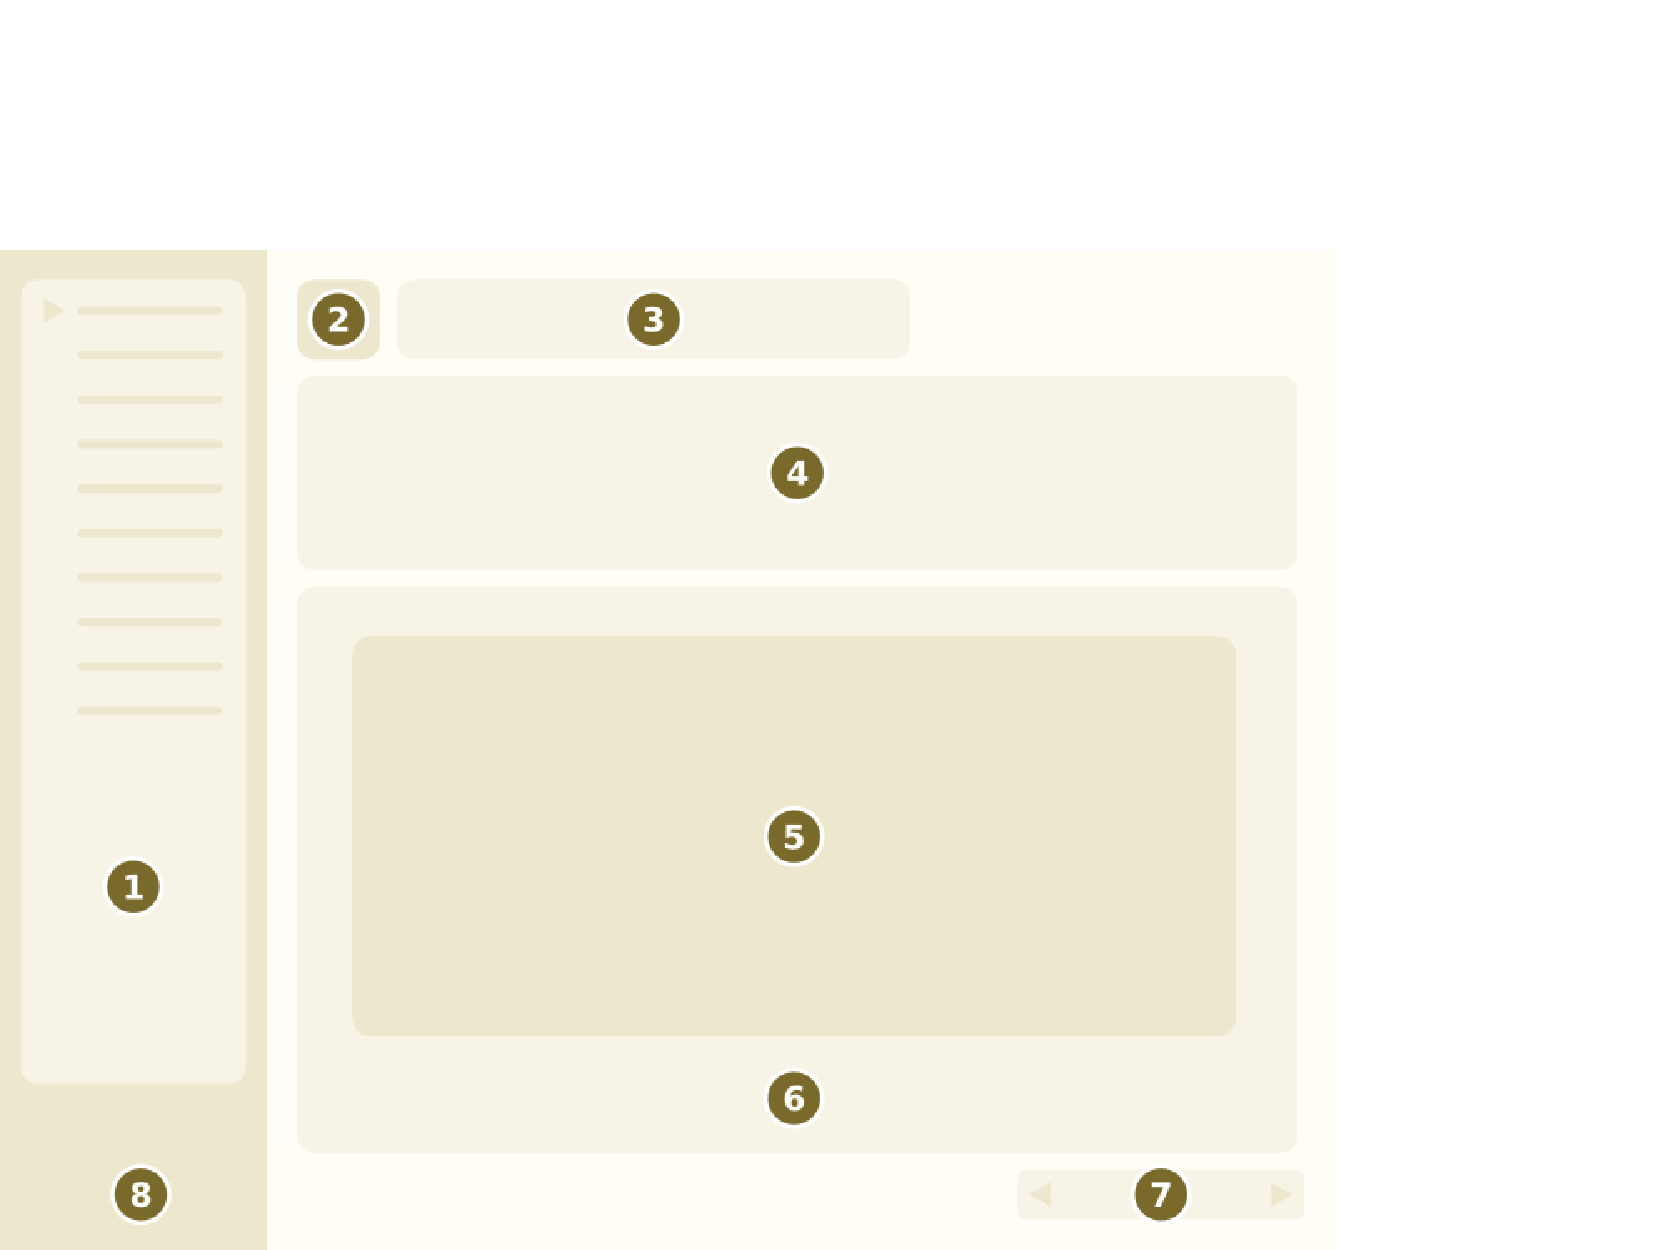
\includegraphics[width=0.8\textwidth]{%
../Identity/Models/Img/en/Distro/Anaconda/Firstboot/splash-small.pdf}}
\end{center}
\caption{Firstboot design model.%
   \label{fig:Distribution:Anaconda:Firstboot:Identity:Models}}
\end{figure}

\begin{description}

\item[1:] List of labels and a pointer showing in which configuration
screen you are.

\item[2:] Screen icon. The screen icon is visible in all firstboot
screens. Each firsboot screen may have its own screen icon.

\item[3:] Screen label.

\item[4:] Screen description. 

\item[5:] Splash image (splash-small.png). The splash
image is visible in firstboot welcome screen only.

\item[6:] Configuration stuff.

\item[7:] Navigation area. Basically two buttons to navegate
configuration back and forward.

\item[8:] List of labels' background image (firtboot-left.png).  This
image is visible in all firstboot screens.

\end{description}

\subsection{Image Files}
\hypertarget{sec:Distribution:Anaconda:Firstboot:Identity:Images}{}
\label{sec:Distribution:Anaconda:Firstboot:Identity:Images}

\begin{description}
\item[framework:]
trunk/Identity/Themes/\$THEME/Distro/Anaconda/Firstboot/Img/
\end{description}

\noindent Here is where firstboot final images are stored. 

\subsection{Image Files Rendering}
\hypertarget{sec:Distribution:Anaconda:Firstboot:Identity:ImagesRendering}{}
\label{sec:Distribution:Anaconda:Firstboot:Identity:ImagesRendering}

\begin{description}
\item[framework:]
trunk/Identity/Themes/\$THEME/Distro/Anaconda/Firstboot/
\end{description}

\noindent Here is where you produce firstboot images. The following
rendering examples, based on
\autoref{fig:Distribution:Anaconda:Firstboot:Translations}, illustrate
the firstboot image files rendering process.\\
\\
\fbox{\texttt{./render.sh}}\\
\\
\fbox{\texttt{./render.sh '(5|6)/splash'}}\\
\\
\fbox{\texttt{./render.sh '(firstboot-left|5|4)/splash'}}

\section{Translations}
\hypertarget{sec:Distribution:Anaconda:Firstboot:Translations}{}
\label{sec:Distribution:Anaconda:Firstboot:Translations}

\begin{description}
\item[framework:]
trunk/Translations/Identity/Themes/Distro/Anaconda/Firstboot
\end{description}

\noindent Here is where translators locale firstboot images. Image
localization is defined inside .sed files, also known as translation
files.  Translation files can be common or specific. The given
organization of translation files defines the translation path.

\begin{figure}[!hbp]
\hrulefill
\begin{verbatim}
trunk/Translations/Identity/Themes/Distro/Anaconda/Firstboot
|-- 3
|   `-- splash-small.sed
|-- 4
|   `-- splash-small.sed
|-- 5
|   `-- splash-small.sed
|-- ... (more release directories)
`-- firstboot-left.sed
\end{verbatim}
\hrulefill
\caption{Firstboot translation path.%
   \label{fig:Distribution:Anaconda:Firstboot:Translations}}
\end{figure}

\subsection{Translation Markers}

In firstboot, markers are used in the file splash-small.svg only,
specifically to set the major release number of CentOS Distribution in
CentOS Release Brand. Since firstboot-left.svg design is common for
all CentOS Distribution there is no need to set any marker on it.

Markers used in firstboot design templates and translation files are
described in \autoref{tab:Distribution:Anaconda:Firstboot:Markers}.

\begin{table}
\centering
\begin{tabular}{rl}
\hline
\textbf{Marker} & \textbf{Description}\\
\hline
=MAJOR\_RELEASE= & Major release number of CentOS Distribution.\\
\hline
\end{tabular}
\caption{Firstboot translation markers.%
   \label{tab:Distribution:Anaconda:Firstboot:Markers}}
\end{table}

\section{Manuals}
\hypertarget{sec:Distribution:Anaconda:Firstboot:Manuals}{}
\label{sec:Distribution:Anaconda:Firstboot:Manuals}

\begin{description}
\item[framework:]
trunk/Manuals/Distribution/Anaconda/Firstboot/
\end{description}

\noindent Here is where firstboot documentation is stored.  If you
want to help improving Firstboot documentation this is the place you
need to go.

\section{Scripts}
\hypertarget{sec:Distribution:Anaconda:Firstboot:Scripts}{}

\begin{description}
\item[framework:] trunk/Scripts/Config/Identity/Themes/Distro/Anaconda/Firstboot/
\end{description}

\noindent Here is stored the Firstboot \texttt{render.conf.sh}
configuration script.  To render Firstboot images correctly, the
\texttt{ARTCOMP} configuration variable inside Anaconda progress
configuration script should be defined as illustrated in
\autoref{fig:Distribution:Anaconda:Firstboot:Scripts:Config}. 

\begin{figure}
\hrulefill
\begin{verbatim}
# Define artwork component.
ARTCOMP='Identity/Themes/Distro/Anaconda/Firstboot'
\end{verbatim}
\hrulefill
\caption{Firstboot configuration layout.%
   \label{fig:Distribution:Anaconda:Firstboot:Scripts:Config}}
\end{figure}


% Part   : Concepts
% Chapter: Rebranding
% ------------------------------------------------------------
% $Id: rebranding.tex 6191 2010-08-02 02:36:14Z al $
% ------------------------------------------------------------

To comply with upstream redistribution policy, the CentOS Project
removes all upstream brands and artworks from CentOS Distribution. The
CentOS Project has its own brand and its own artwork. The CentOS Brand
and CentOS Artwork are what the CentOS Project uses in CentOS
Distribution. 

The action of removing upstream brands and artworks and add CentOS
brands and artworks is what we call rebranding.

CentOS Brands and artworks are organized inside CentOS Artwork
Repository.  The CentOS Artwork Repository is maintain by CentOS
Artwork SIG which is formed by CentOS Community People.

\section{General Suggestions}

\begin{itemize}

\item Use original names as much as possible. Do not rename original
file names if you don't need to.

\end{itemize}



\input{../../../../../Licenses/GFDL.tex}

\end{document}
